\begin{figure}[t]

\rkc{Move all this code into the mockup screenshots below.}

\lstset{basicstyle=\scriptsize\ttfamily}
\begin{lstlisting}
type grade_cutoffs =
  { a: float, b: float, c: float, d: float, f: float };

let cutoffs =
  { a = ??_a, b = ??_b, c = ??_c, d = ??_d, f = ??_f };

let letter_grade(n: weighted_average) =
  if n >= cutoffs.a then "A" else
  if n >= cutoffs.b then "B" else
  if n >= cutoffs.c then "C" else
  if n >= cutoffs.d then "D" else
  if n >= cutoffs.f then "F" else "Incomplete";

let sorted_weighted_averages = List.sort weighted_averages;

let letter_grades = List.map letter_grade sorted_weighted_averages;

let compute_distribution(list: list(float)) =
  let n = List.length letter_grades in
  List.map
    (\x -> (x, showPercentage (List.length (List.filter ((==) x) list)) /. n))
    ["A","B","C","D","F","Incomplete"];

let distribution = compute_distribution(letter_grades);
\end{lstlisting}
%% restore settings from main.tex
\lstset{basicstyle=\footnotesize\ttfamily}

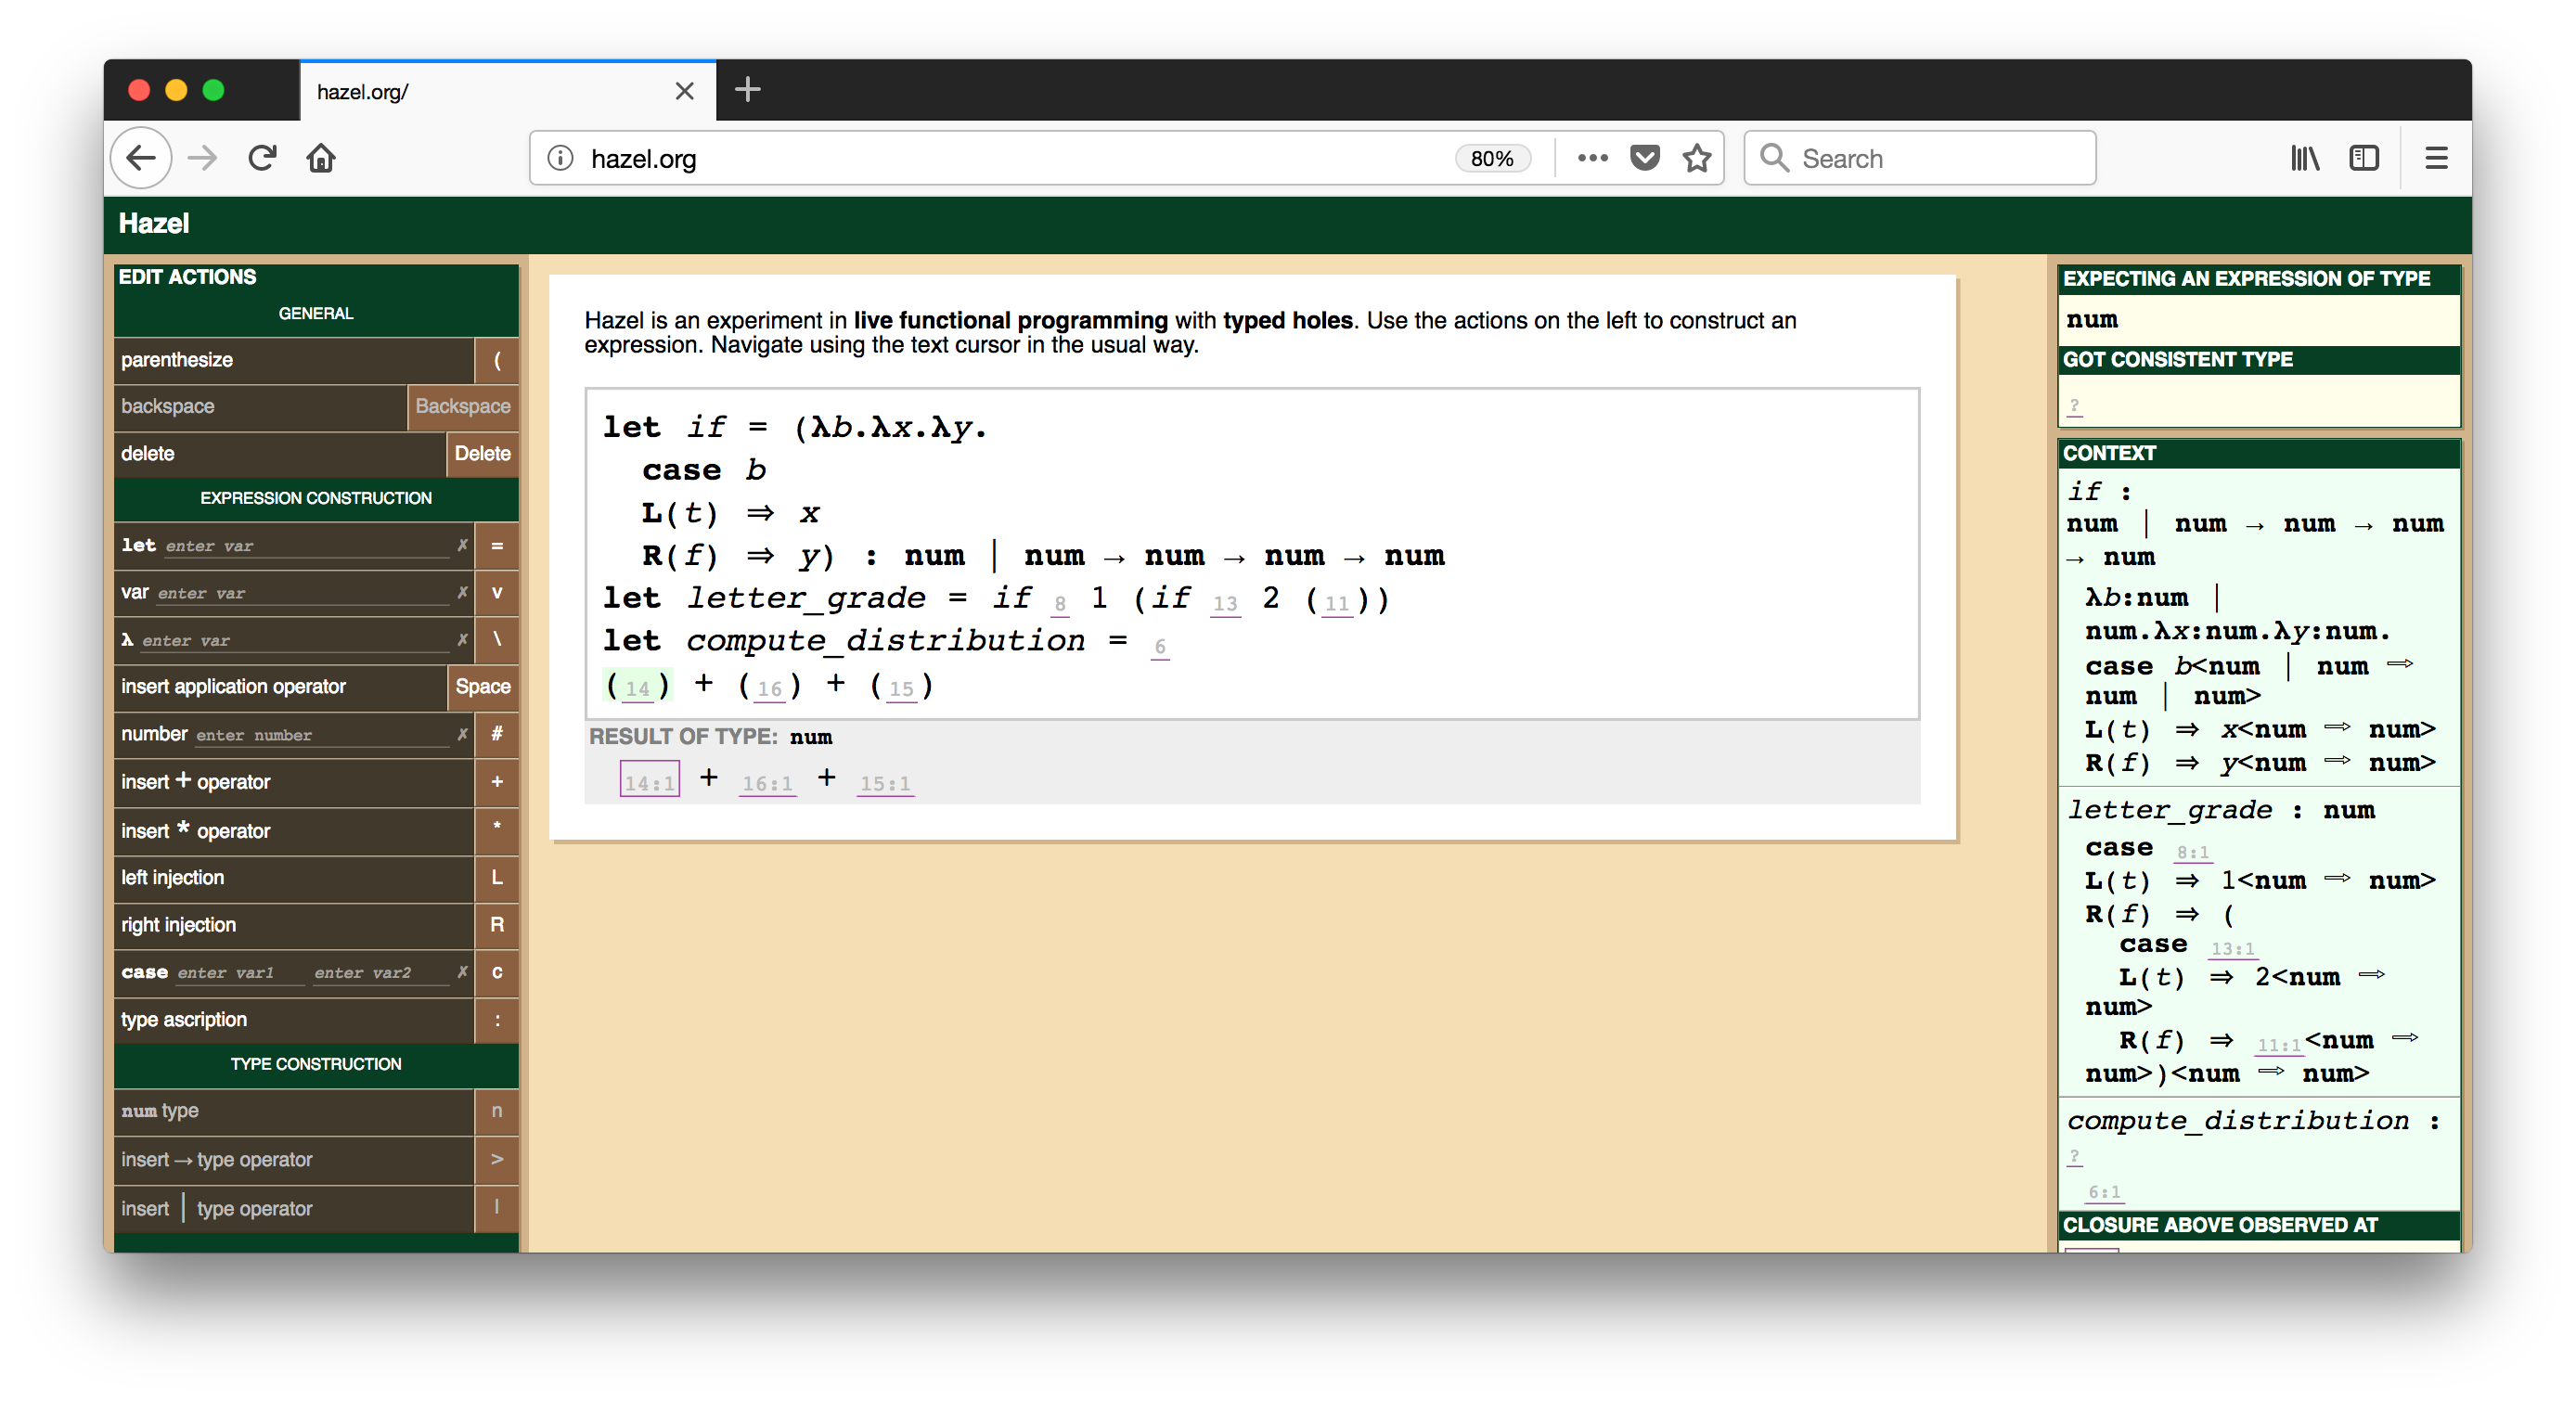
\includegraphics[scale=0.27]{images/hazel-placeholder-1b.png}

\caption{Hazel mockup for Example 1b.}
\label{fig:grades-example-b}
\end{figure}
